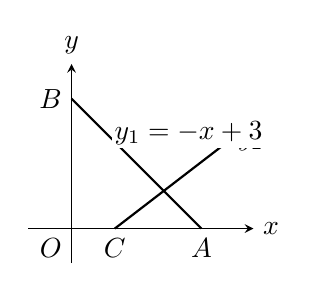
\begin{tikzpicture}[scale=0.55,>=stealth]
  \draw[->] (-1,0)--(4.2,0) node[right] {$x$};
  \draw[->] (0,-0.8)--(0,3.8) node[above] {$y$};
  \draw[thick] (0,3)--(3,0) node[below] {$A$};
  \node[left] at (0,3) {$B$};
  \node[below left] at (0,0) {$O$};
  \draw[thick] (1,0)--(3.6,2.0) node[right] {$y_2$};
  \node[below] at (1,0) {$C$};
  \node[fill=white,inner sep=1pt] at (2.7,2.2) {$y_1=-x+3$};
\end{tikzpicture}
